% Options for packages loaded elsewhere
\PassOptionsToPackage{unicode}{hyperref}
\PassOptionsToPackage{hyphens}{url}
\documentclass[
  ignorenonframetext,
]{beamer}
\newif\ifbibliography
\usepackage{pgfpages}
\setbeamertemplate{caption}[numbered]
\setbeamertemplate{caption label separator}{: }
\setbeamercolor{caption name}{fg=normal text.fg}
\beamertemplatenavigationsymbolsempty
% remove section numbering
\setbeamertemplate{part page}{
  \centering
  \begin{beamercolorbox}[sep=16pt,center]{part title}
    \usebeamerfont{part title}\insertpart\par
  \end{beamercolorbox}
}
\setbeamertemplate{section page}{
  \centering
  \begin{beamercolorbox}[sep=12pt,center]{section title}
    \usebeamerfont{section title}\insertsection\par
  \end{beamercolorbox}
}
\setbeamertemplate{subsection page}{
  \centering
  \begin{beamercolorbox}[sep=8pt,center]{subsection title}
    \usebeamerfont{subsection title}\insertsubsection\par
  \end{beamercolorbox}
}
% Prevent slide breaks in the middle of a paragraph
\widowpenalties 1 10000
\raggedbottom
\AtBeginPart{
  \frame{\partpage}
}
\AtBeginSection{
  \ifbibliography
  \else
    \frame{\sectionpage}
  \fi
}
\AtBeginSubsection{
  \frame{\subsectionpage}
}
\usepackage{iftex}
\ifPDFTeX
  \usepackage[T1]{fontenc}
  \usepackage[utf8]{inputenc}
  \usepackage{textcomp} % provide euro and other symbols
\else % if luatex or xetex
  \usepackage{unicode-math} % this also loads fontspec
  \defaultfontfeatures{Scale=MatchLowercase}
  \defaultfontfeatures[\rmfamily]{Ligatures=TeX,Scale=1}
\fi
\usepackage{lmodern}
\ifPDFTeX\else
  % xetex/luatex font selection
\fi
% Use upquote if available, for straight quotes in verbatim environments
\IfFileExists{upquote.sty}{\usepackage{upquote}}{}
\IfFileExists{microtype.sty}{% use microtype if available
  \usepackage[]{microtype}
  \UseMicrotypeSet[protrusion]{basicmath} % disable protrusion for tt fonts
}{}
\makeatletter
\@ifundefined{KOMAClassName}{% if non-KOMA class
  \IfFileExists{parskip.sty}{%
    \usepackage{parskip}
  }{% else
    \setlength{\parindent}{0pt}
    \setlength{\parskip}{6pt plus 2pt minus 1pt}}
}{% if KOMA class
  \KOMAoptions{parskip=half}}
\makeatother
\usepackage{graphicx}
\makeatletter
\newsavebox\pandoc@box
\newcommand*\pandocbounded[1]{% scales image to fit in text height/width
  \sbox\pandoc@box{#1}%
  \Gscale@div\@tempa{\textheight}{\dimexpr\ht\pandoc@box+\dp\pandoc@box\relax}%
  \Gscale@div\@tempb{\linewidth}{\wd\pandoc@box}%
  \ifdim\@tempb\p@<\@tempa\p@\let\@tempa\@tempb\fi% select the smaller of both
  \ifdim\@tempa\p@<\p@\scalebox{\@tempa}{\usebox\pandoc@box}%
  \else\usebox{\pandoc@box}%
  \fi%
}
% Set default figure placement to htbp
\def\fps@figure{htbp}
\makeatother
\setlength{\emergencystretch}{3em} % prevent overfull lines
\providecommand{\tightlist}{%
  \setlength{\itemsep}{0pt}\setlength{\parskip}{0pt}}
% Slide layout defaults for warning-clean scientific decks.
\usepackage{etoolbox}
\IfFileExists{xurl.sty}{\usepackage{xurl}}{}
\IfFileExists{seqsplit.sty}{\usepackage{seqsplit}}{\newcommand{\seqsplit}[1]{#1}}
\protected\def\breakseq#1{\seqsplit{#1}}
\protected\def\breaktt#1{\begingroup\ttfamily\seqsplit{#1}\endgroup}
\setlength{\emergencystretch}{6em}
\tolerance=5000
\hbadness=10000
\hfuzz=1pt
\setlength{\tabcolsep}{2pt}
\AtBeginEnvironment{longtable}{\tiny\renewcommand{\arraystretch}{0.86}\setlength{\tabcolsep}{1pt}}
\AtBeginEnvironment{tabular}{\tiny\renewcommand{\arraystretch}{0.86}\setlength{\tabcolsep}{1pt}}

% Natbib and cross-reference fallbacks — slides don't load natbib
% or cleveref, but combined-PDF manuscript prose may emit these
% commands. The fallback renders citations as a bracketed key list
% and cross-references as detokenized labels so slides don't fail on
% undefined control sequences or raw underscores. \providecommand is
% a no-op if packages load later.
\providecommand{\citep}[1]{[#1]}
\providecommand{\citet}[1]{#1}
\providecommand{\citealp}[1]{#1}
\providecommand{\citeauthor}[1]{#1}
\providecommand{\citeyear}[1]{#1}
\providecommand{\cref}[1]{\texttt{\detokenize{#1}}}
\providecommand{\Cref}[1]{\texttt{\detokenize{#1}}}

\newtheorem{proposition}{Proposition}
\newtheorem{hypothesis}{Hypothesis}
\usepackage{bookmark}
\IfFileExists{xurl.sty}{\usepackage{xurl}}{} % add URL line breaks if available
\urlstyle{same}
% fallback for those not using the hyperref driver hyperxmp:
\makeatletter
\@ifundefined{xmpquote}{\newcommand{\xmpquote}[1]{#1}}{}
\makeatother
\hypersetup{
  hidelinks,
  pdfcreator={LaTeX via pandoc}}

\author{\texorpdfstring{}{}}
\date{}

\begin{document}

\section{Appendix: Free-Energy and Active-Inference
Formalisms}\label{sec:formalisms_appendix}

\begin{frame}[allowframebreaks]{Appendix: Free-Energy and
Active-Inference Formalisms}
This appendix holds the mathematical and diagnostic primitives used by
the main manuscript. The consolidation is deliberate: active inference
remains a modeling lens in the main line, while the formal details sit
here where readers can inspect assumptions, generators, labels, and
evidence boundaries together. The appendix draws on established
active-inference and free-energy treatments \breakseq{[@friston2010fep;
@friston2017process; @parr2022activeinference; @friston2023simpler]},
discrete-state synthesis work \breakseq{[@dacosta2020discrete]}, and
interactional accounts of communication and second-person modeling
\breakseq{[@vasil2020communication; @schilbach2013secondperson;
@redcay2019secondperson; @bolis2024secondperson]}.
\end{frame}

\begin{frame}[fragile,allowframebreaks]{Event-to-Model Mapping}
\protect\phantomsection\label{event-to-model-mapping}
\breakseq{[@fig:active\_inference\_mapping]} maps DigiPPPiP's theoretical terms
to observable design elements. Latent states are partner intentions,
narrative states, and shared affect. Observations are strokes, pauses,
utterances, and interface events. Policies are drawing, waiting,
responding, and revising. The figure is included to prevent active
inference from becoming decorative terminology: every model term has to
be tied to a protocol event or dropped.

\begin{figure}
\centering
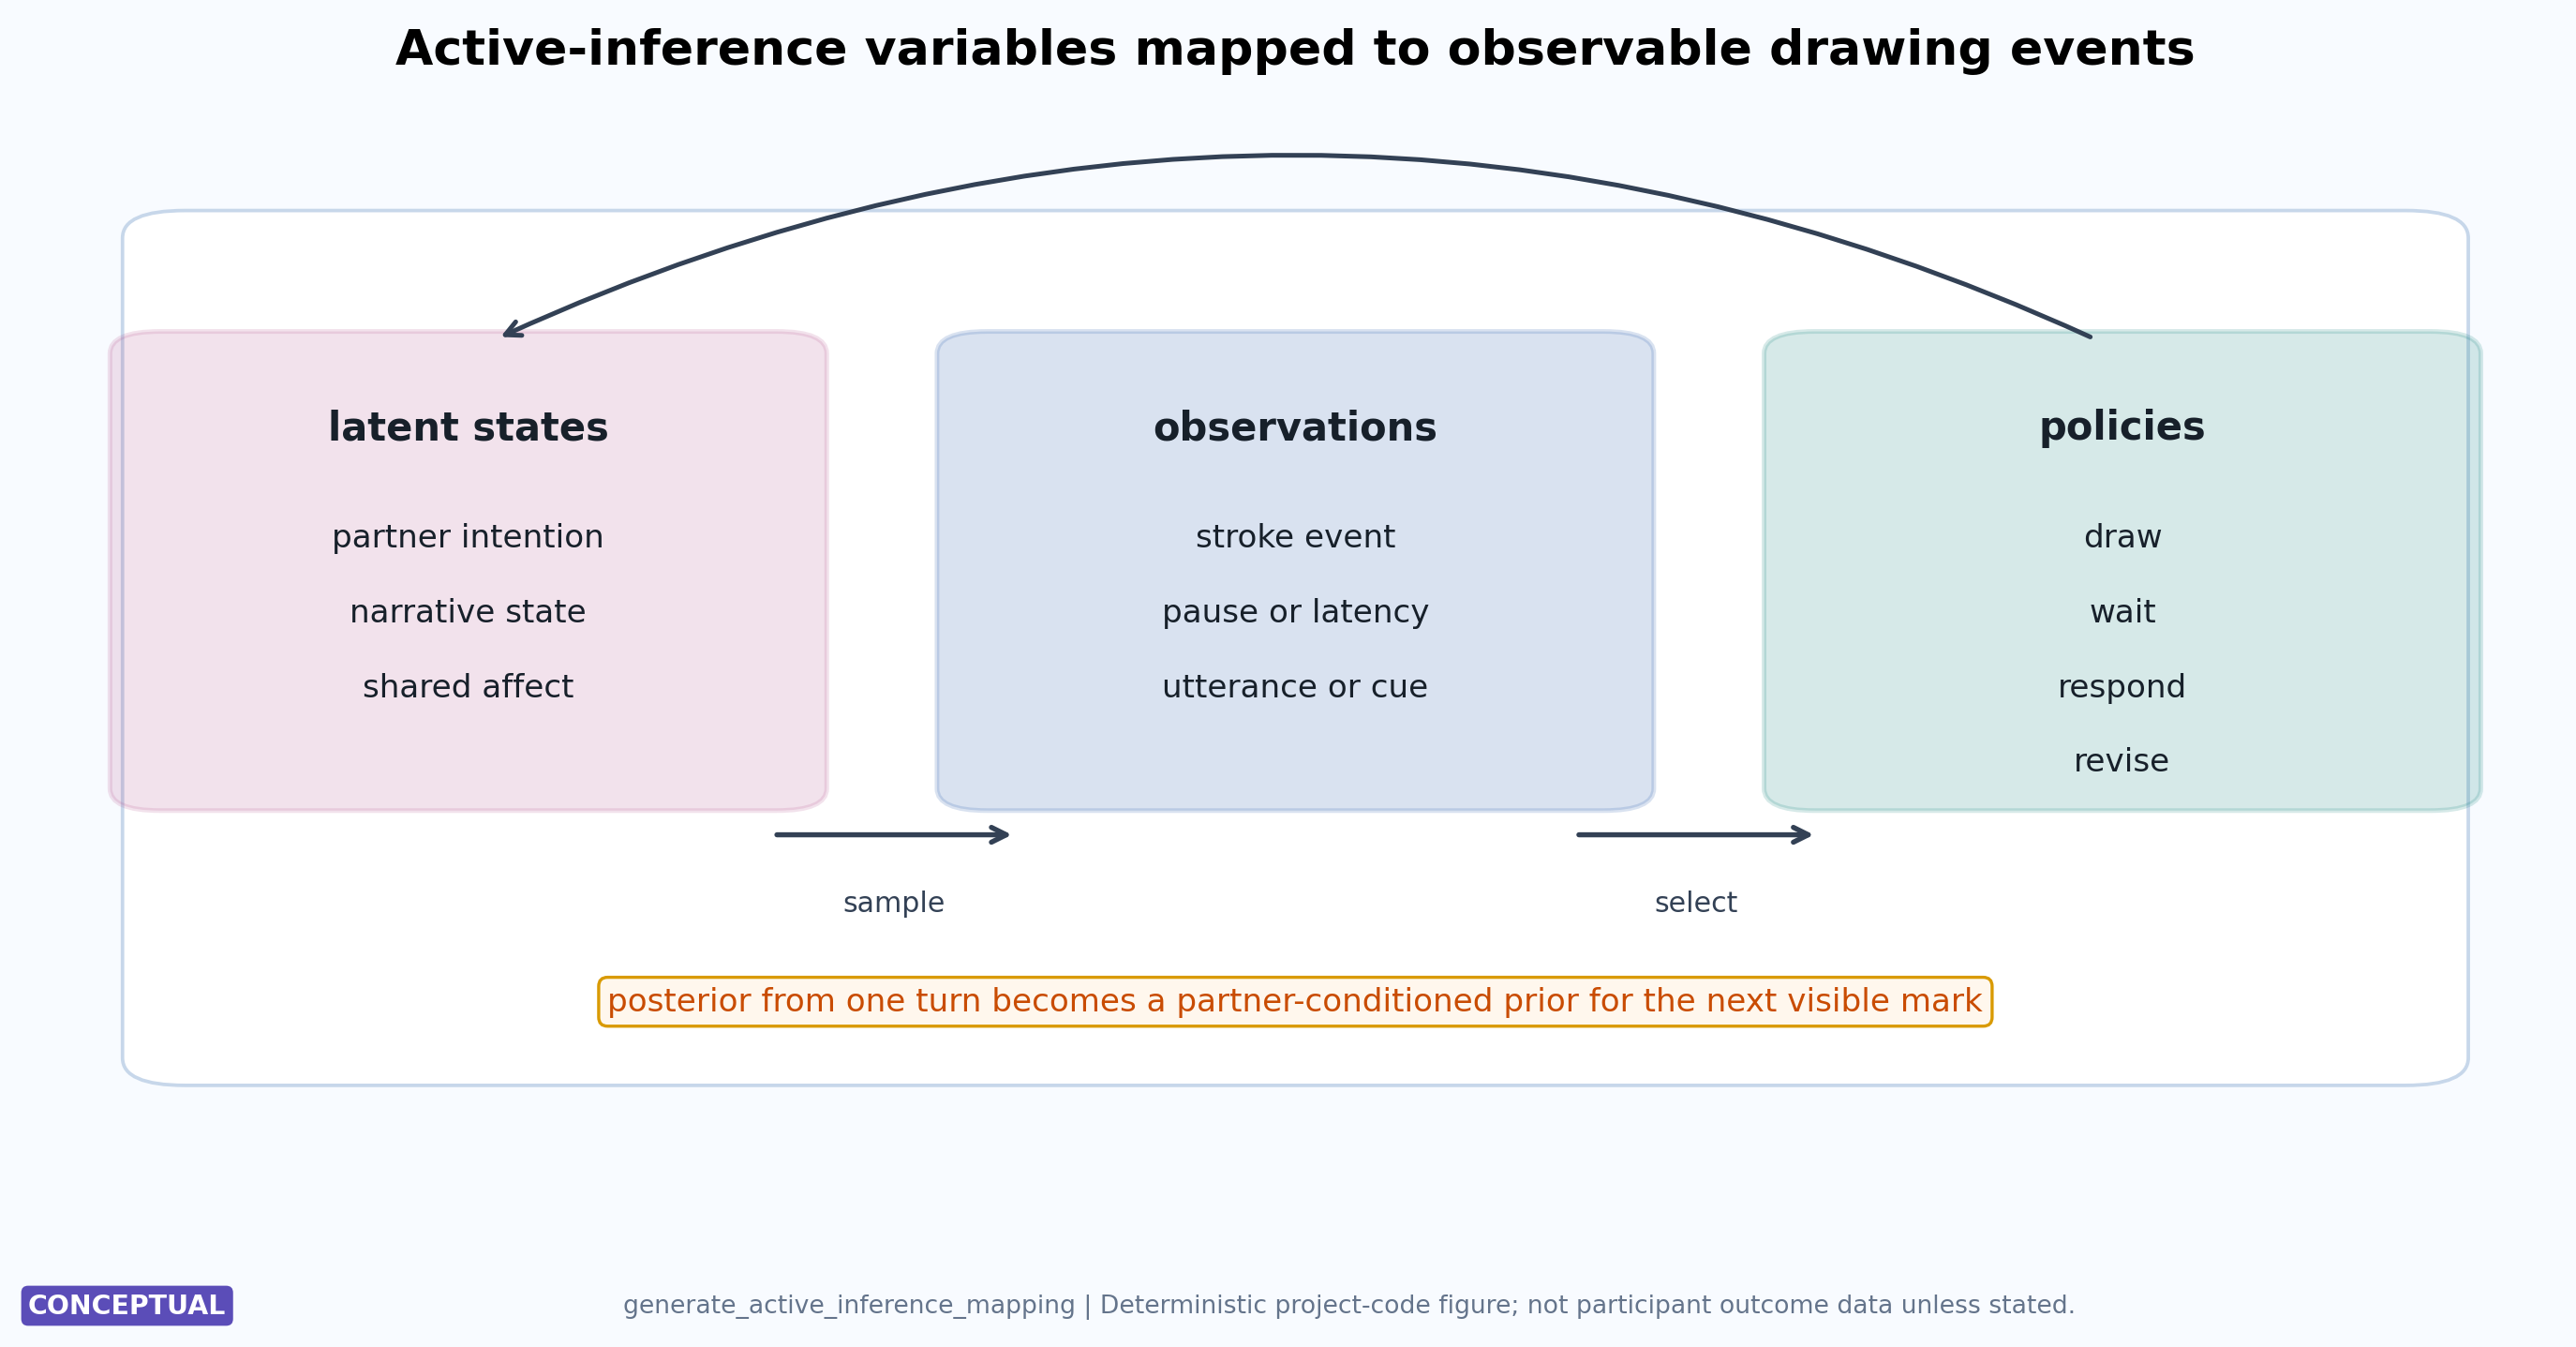
\includegraphics[width=0.9\linewidth,height=0.46\textheight,keepaspectratio,alt={Mapping from DigiPPPiP events to active-inference model components. The figure is generated by generate\_active\_inference\_mapping(); read the columns as latent states, observations, and policies, with arrows showing how partner-conditioned beliefs can update through visible marks. It supports the active-inference appendix by tying terms to measurable protocol events. The mapping is conceptual; fitted parameters and failed-baseline checks would be needed for mechanism claims.}]{../figures/active_inference_mapping.png}
\caption{Mapping from DigiPPPiP events to active-inference model
components. The figure is generated by
\protect\breaktt{generate\_active\_inference\_mapping()}; read the
columns as latent states, observations, and policies, with arrows
showing how partner-conditioned beliefs can update through visible
marks. It supports the active-inference appendix by tying terms to
measurable protocol events. The mapping is conceptual; fitted parameters
and failed-baseline checks would be needed for mechanism
claims.}\label{fig:active_inference_mapping}
\end{figure}
\end{frame}

\begin{frame}[fragile,allowframebreaks]{Minimal Free-Energy Primitive}
\protect\phantomsection\label{minimal-free-energy-primitive}
The project uses a Gaussian point-belief model as a minimal conceptual
primitive. Variational free energy is:

\[
F(\mu)=\frac{1}{2}\pi_p(\mu-\mu_p)^2+\frac{1}{2}\pi_l(o-\mu)^2-\frac{1}{2}\log \pi_p-\frac{1}{2}\log \pi_l
\] \{\#eq:vfe\}

The expression in \breakseq{[@eq:vfe]} defines \(\mu\) as the current belief,
\(\mu_p\) as the prior mean, \(o\) as the canvas observation, and
\(\pi_p,\pi_l\) as the prior and likelihood precisions. The analytic
posterior mean used by \breaktt{src/active\_inference.py} is:

\[
\mu^\ast=\frac{\pi_p\mu_p+\pi_l o}{\pi_p+\pi_l}
\] \{\#eq:posterior\}

In a coupled dyad, each partner's previous posterior becomes part of the
other's next prior. \breakseq{[@fig:active\_inference\_loop]} contrasts that
coupled case with a decoupled baseline. The terminal free-energy values
from the deterministic conceptual run are -0.693147 and 0.061153,
respectively; the absolute reduction is 0.7543. These are model outputs,
not human-subject measurements.

\begin{figure}
\centering
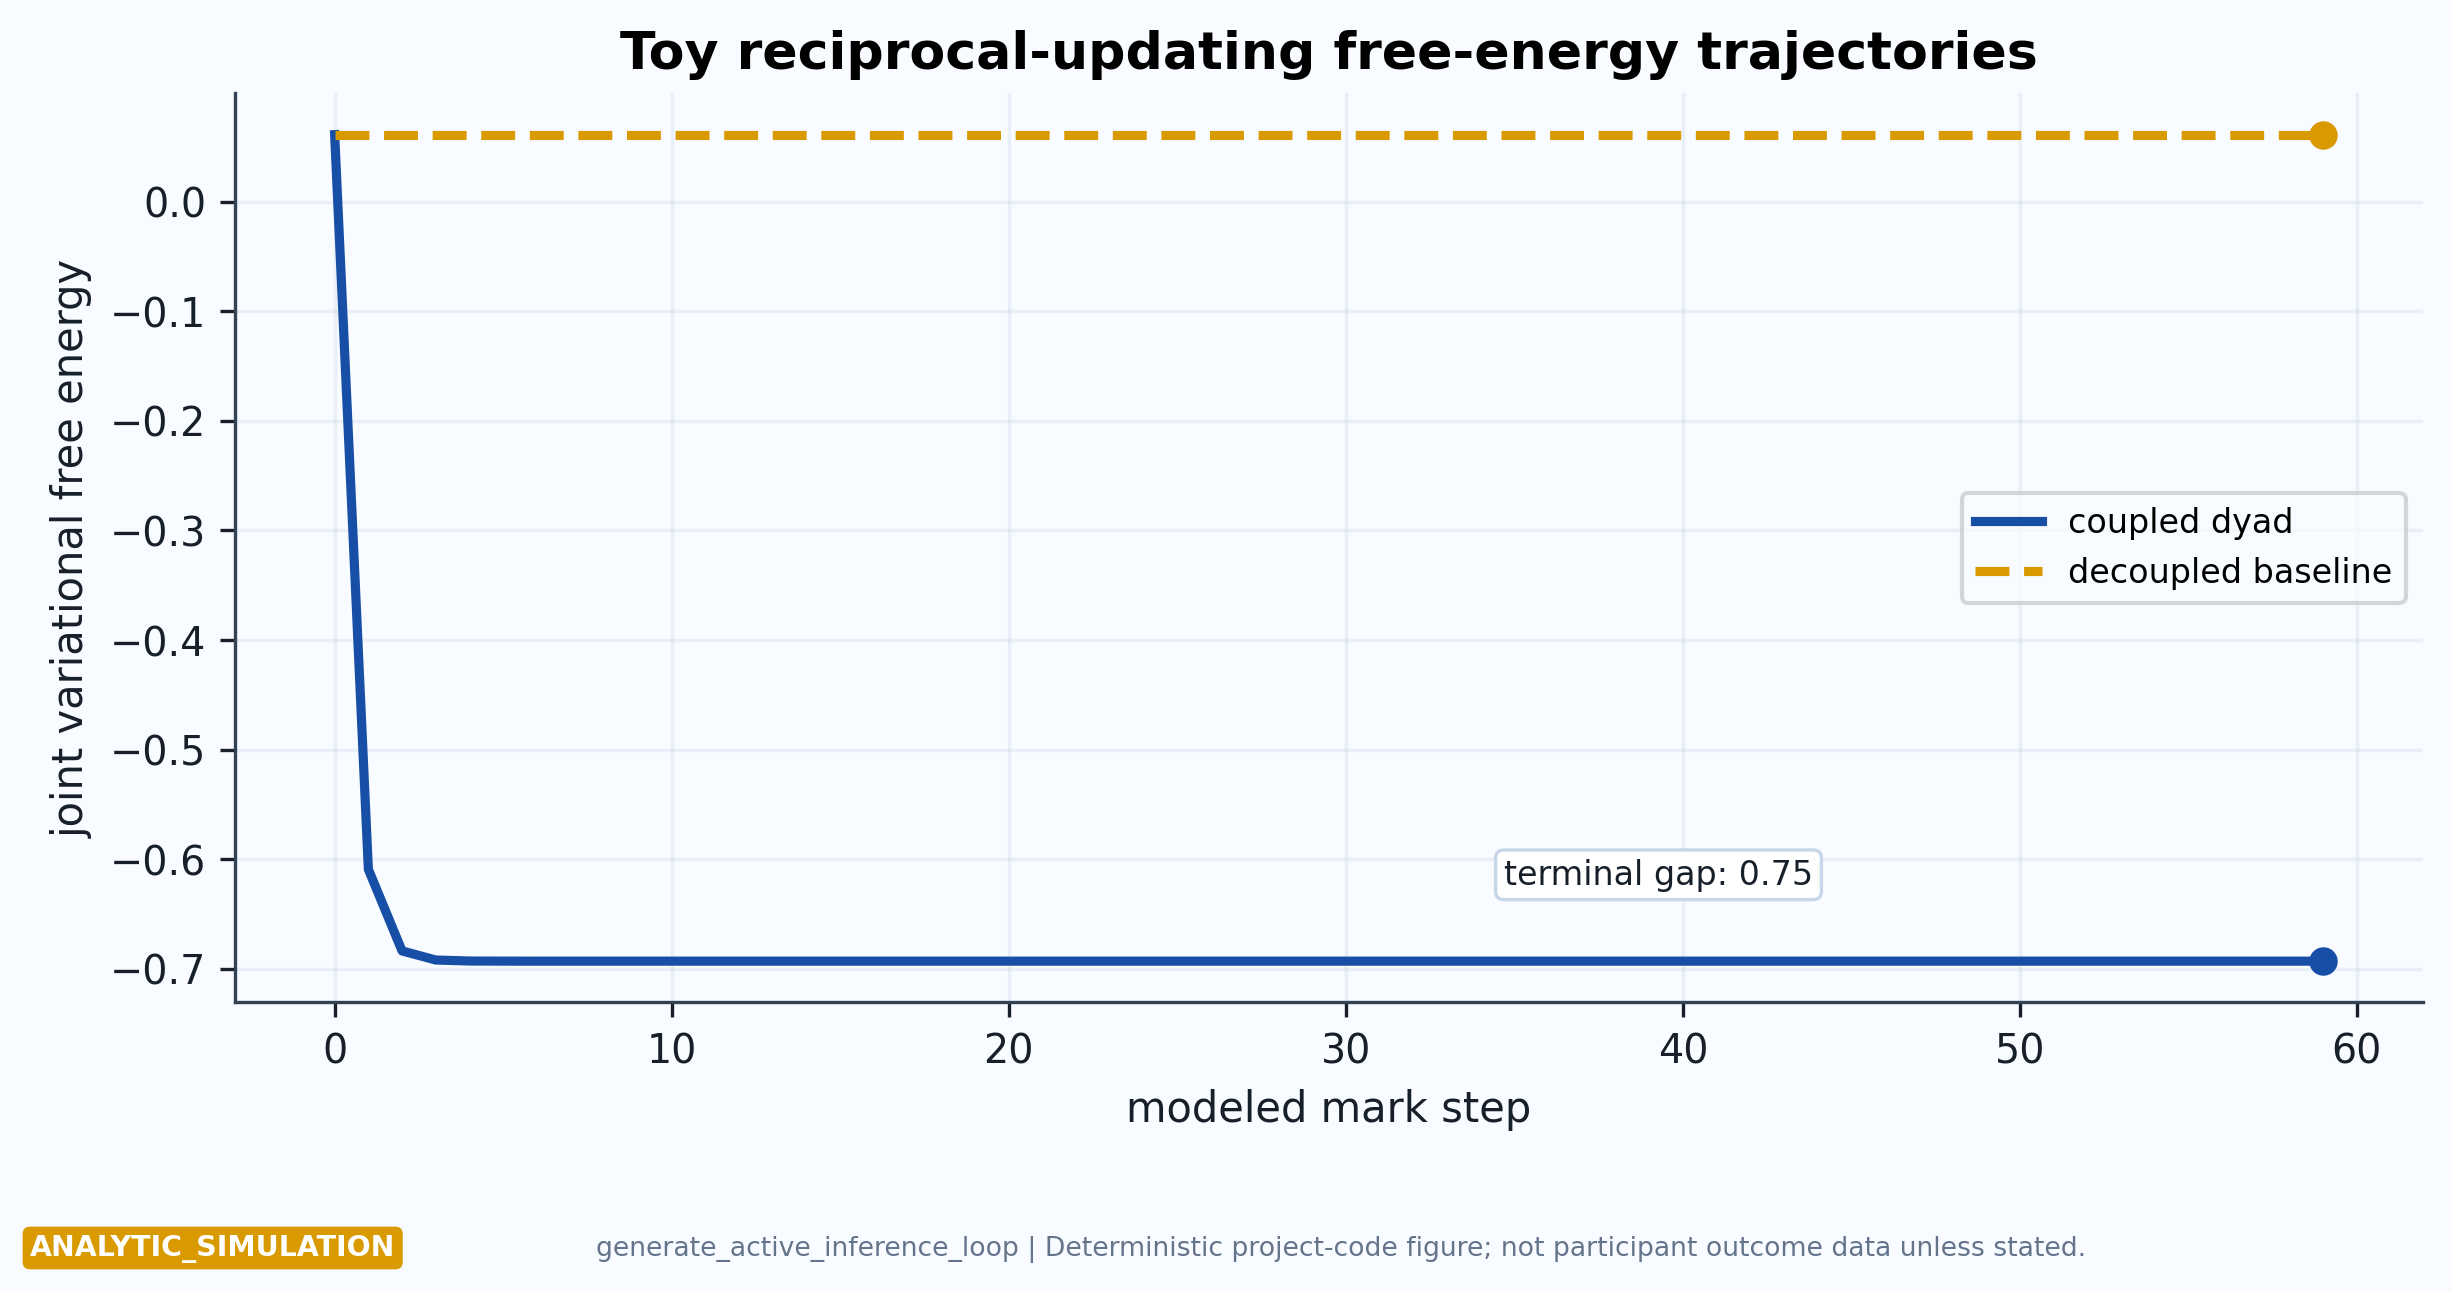
\includegraphics[width=0.9\linewidth,height=0.46\textheight,keepaspectratio,alt={Coupled and decoupled conceptual free-energy trajectories generated by generate\_active\_inference\_loop() from simulate\_dyadic\_session(). Read the solid and dashed lines as toy-model baselines for reciprocal versus non-reciprocal prior updating across mark steps. The plot supports the modeling argument that coupling can be formalized, not that couples improve. Empirical validation would require observed behavior and model-comparison evidence.}]{../figures/active_inference_loop.png}
\caption{Coupled and decoupled conceptual free-energy trajectories
generated by \protect\breaktt{generate\_active\_inference\_loop()} from
\protect\breaktt{simulate\_dyadic\_session()}. Read the solid and dashed
lines as toy-model baselines for reciprocal versus non-reciprocal prior
updating across mark steps. The plot supports the modeling argument that
coupling can be formalized, not that couples improve. Empirical
validation would require observed behavior and model-comparison
evidence.}\label{fig:active_inference_loop}
\end{figure}
\end{frame}

\begin{frame}[fragile,allowframebreaks]{Hyperscanning and Network
Geometry}
\protect\phantomsection\label{hyperscanning-and-network-geometry}
Geometric hyperscanning is a candidate measurement vocabulary for
empirical studies, not a shortcut to interpreting synchrony.
Near-infrared spectroscopy (NIRS)-based cooperation studies and
hyperscanning reviews motivate dyadic measurement \breakseq{[@cui2012nirs;
@czeszumski2020hyperscanning; @czeszumski2022cooperative;
@nam2020hyperscanningreview]}, yet shared stimulus timing, motion
artifacts, physiology, task structure, preprocessing choices, and
analytic windows can all inflate apparent coupling. Methodological
cautions in fNIRS and hyperscanning warn against interpreting
cross-brain coherence as direct evidence of shared minds, empathy, or
relationship improvement \breakseq{[@tachtsidis2016fnirs;
@hamilton2021hyperscanning; @zimmermann2024methodological]}.
Translational hyperscanning arguments are valuable only when they remain
close to applied contexts and family or dyadic care questions rather
than treating synchrony as a generic marker of social quality
\breakseq{[@provenzi2022translational]}. \breakseq{[@fig:network\_analysis\_pipeline]}
therefore separates acquisition, cleaning, windowing, synchrony
estimation, graph construction, and curvature analysis before
interpretation.

\begin{figure}
\centering
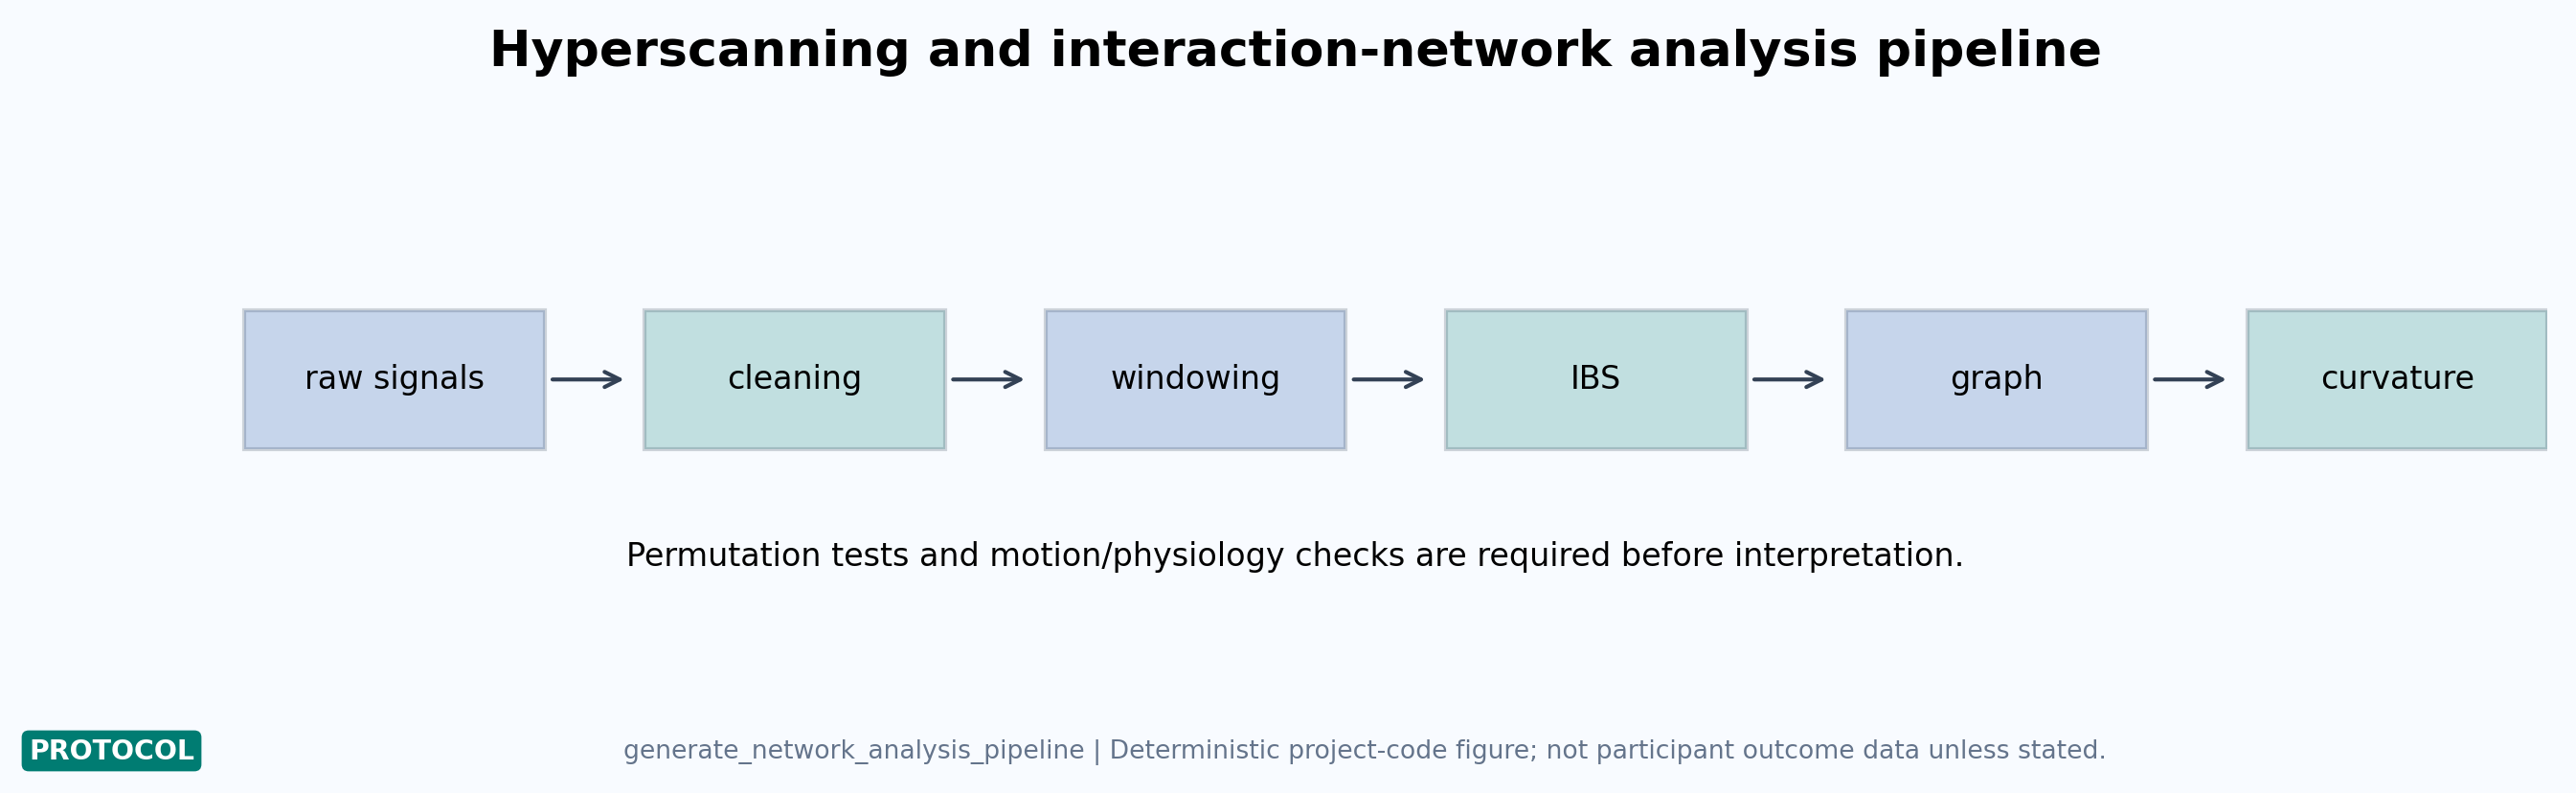
\includegraphics[width=0.9\linewidth,height=0.46\textheight,keepaspectratio,alt={Reproducible pipeline from raw dyadic signals to interaction-network diagnostics. The figure is generated by generate\_network\_analysis\_pipeline(); read the boxes left to right as acquisition, cleaning, windowing, synchrony estimation, graph construction, and curvature analysis. It supports the methods guardrail that signal processing precedes interpretation. The pipeline is analytic scaffolding; actual studies must report exclusion windows, preprocessing choices, and permutation controls.}]{../figures/network_analysis_pipeline.png}
\caption{Reproducible pipeline from raw dyadic signals to
interaction-network diagnostics. The figure is generated by
\protect\breaktt{generate\_network\_analysis\_pipeline()}; read the boxes
left to right as acquisition, cleaning, windowing, synchrony estimation,
graph construction, and curvature analysis. It supports the methods
guardrail that signal processing precedes interpretation. The pipeline
is analytic scaffolding; actual studies must report exclusion windows,
preprocessing choices, and permutation
controls.}\label{fig:network_analysis_pipeline}
\end{figure}

\breakseq{[@fig:hyperscanning\_alignment]} makes the alignment problem more
concrete. Behavioral events, physiological channels, and exclusion
windows must be synchronized before a study can ask whether a neural
measure tracks co-drawing, repair, rupture, or co-regulation. The figure
deliberately includes a shared artifact window to show how apparent
coupling can arise from non-social signal contamination.

\begin{figure}
\centering
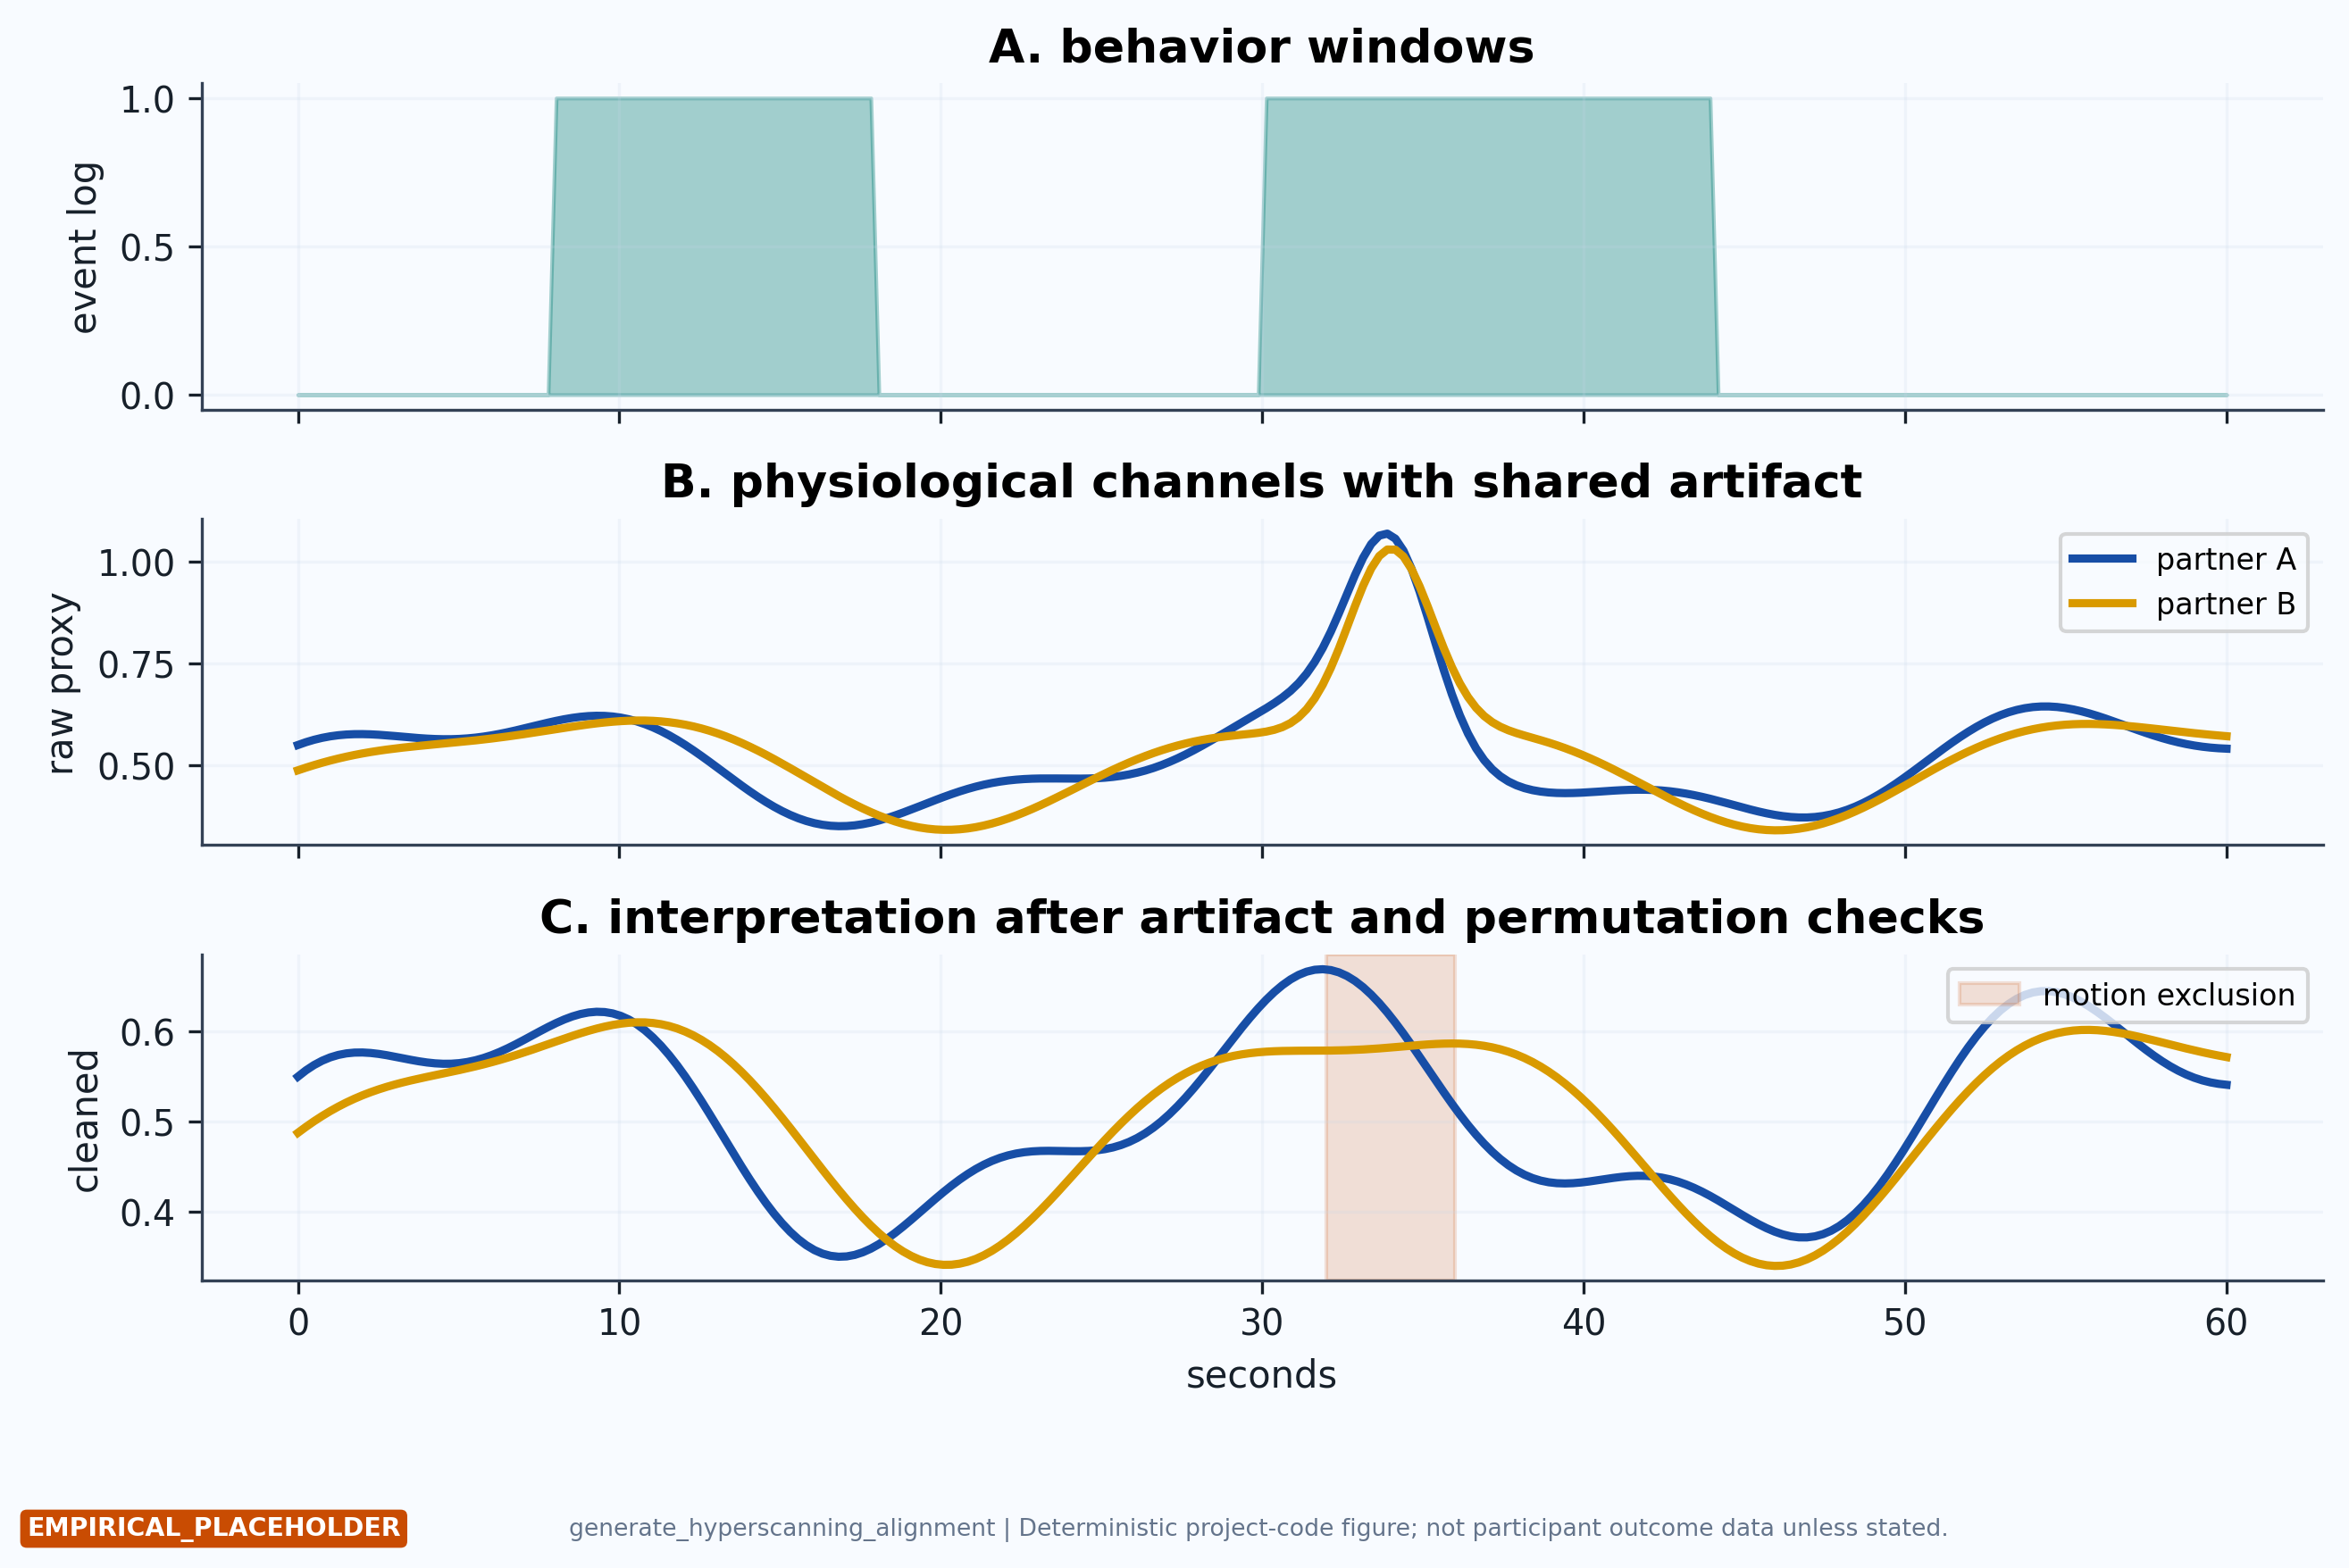
\includegraphics[width=0.9\linewidth,height=0.46\textheight,keepaspectratio,alt={Alignment schematic for behavior, physiology, artifact rejection, and cautious interpretation. The three tracks generated by generate\_hyperscanning\_alignment() should be read vertically: behavioral event windows, raw physiological channels with shared artifacts, and cleaned channels after exclusion. It supports the caution that synchrony claims require co-registration and artifact handling. The signals are simulated; measured analyses would need device-specific quality metrics and null models.}]{../figures/hyperscanning_alignment.png}
\caption{Alignment schematic for behavior, physiology, artifact
rejection, and cautious interpretation. The three tracks generated by
\protect\breaktt{generate\_hyperscanning\_alignment()} should be read
vertically: behavioral event windows, raw physiological channels with
shared artifacts, and cleaned channels after exclusion. It supports the
caution that synchrony claims require co-registration and artifact
handling. The signals are simulated; measured analyses would need
device-specific quality metrics and null
models.}\label{fig:hyperscanning_alignment}
\end{figure}

For a simple unweighted inter-brain graph, the Forman-Ricci curvature
used here is:

\[
\mathrm{Fr}(uv)=4-\deg(u)-\deg(v)
\] \{\#eq:forman\_ricci\}

The implementation uses Forman's cell-complex curvature vocabulary and
dynamic-network change-detection applications as method antecedents
\breakseq{[@forman2003bochner; @weber2016forman]}. The curvature-entropy
diagnostic in \breakseq{[@fig:geometric\_hyperscanning]} follows recent
proposals to treat topological reconfiguration in inter-brain networks
as a marker of affective phase transitions \breakseq{[@hinrichs2025geometric]}.
The conceptual run has maximum curvature entropy 2.4087 and detects 48
transition events under the configured threshold.

\begin{figure}
\centering
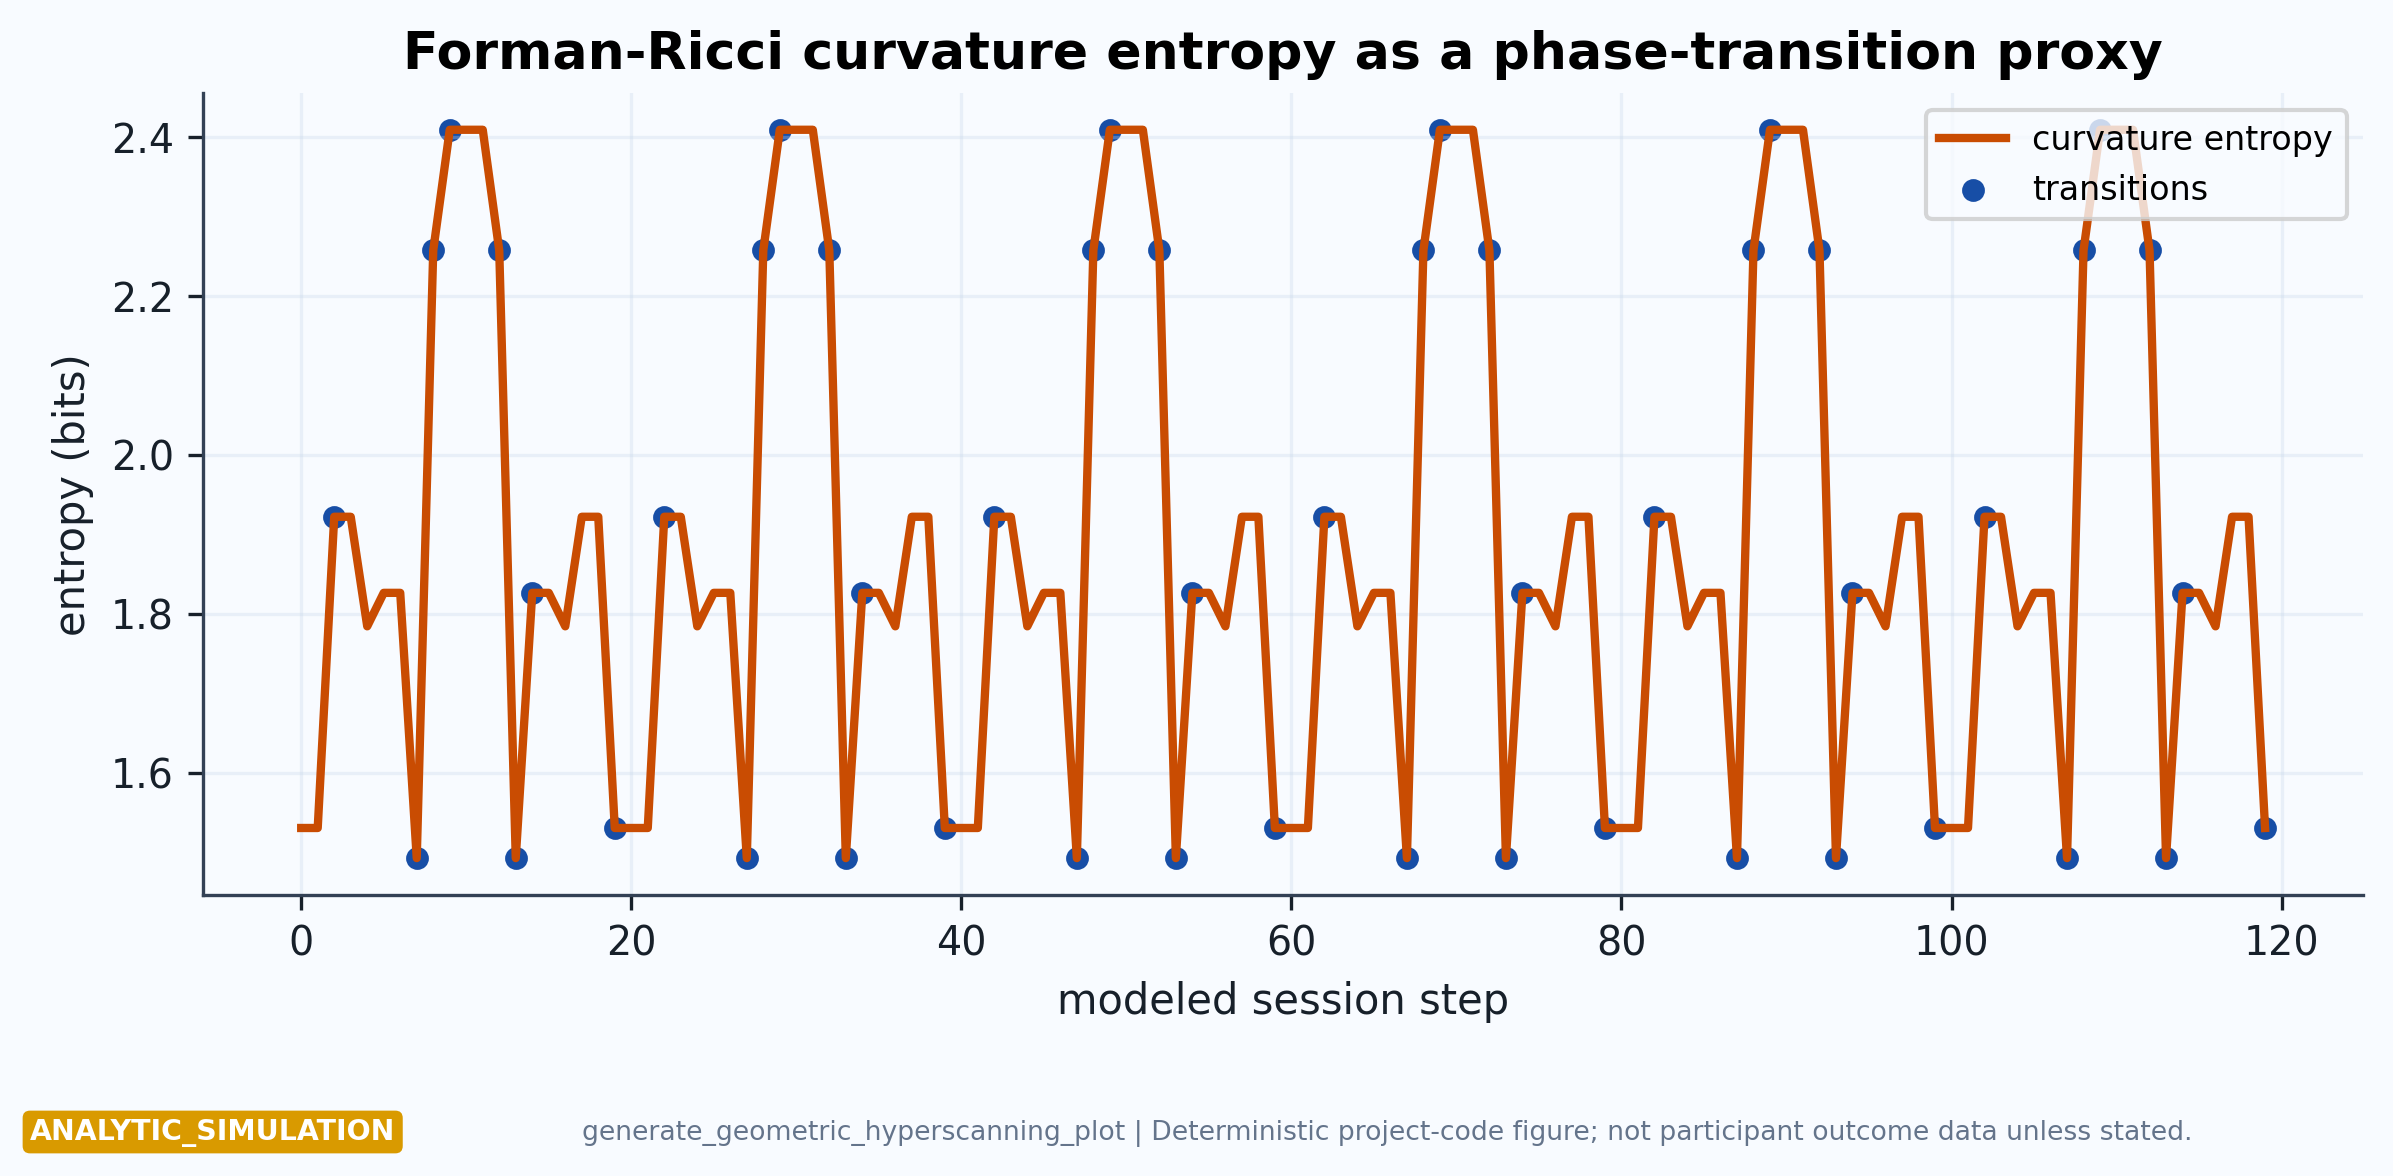
\includegraphics[width=0.9\linewidth,height=0.46\textheight,keepaspectratio,alt={Conceptual curvature entropy over a modeled inter-brain network sequence. The plot is generated by generate\_geometric\_hyperscanning\_plot() from synthetic network snapshots; read the red curve as curvature entropy and blue points as candidate transitions. It supports the proposal that graph diagnostics could mark rupture or repair windows. The figure is not participant hyperscanning, and empirical use would require artifact-robust network estimation.}]{../figures/geometric_hyperscanning.png}
\caption{Conceptual curvature entropy over a modeled inter-brain network
sequence. The plot is generated by
\protect\breaktt{generate\_geometric\_hyperscanning\_plot()} from
synthetic network snapshots; read the red curve as curvature entropy and
blue points as candidate transitions. It supports the proposal that
graph diagnostics could mark rupture or repair windows. The figure is
not participant hyperscanning, and empirical use would require
artifact-robust network estimation.}\label{fig:geometric_hyperscanning}
\end{figure}
\end{frame}

\begin{frame}[fragile,allowframebreaks]{Narrative Information and
Aesthetic Discovery}
\protect\phantomsection\label{narrative-information-and-aesthetic-discovery}
Narrative also fits the active-inference vocabulary. Narratives guide
event segmentation, identity coherence, and policy selection
\breakseq{[@bouizegarene2024narrative; @veisserie2020thinking]}. In DigiPPPiP,
a mark sequence can be treated as a symbolic trajectory with Shannon
entropy and surprisal \breakseq{[@shannon1948mathematical]}:

\[
H(X)=-\sum_i p(x_i)\log_2 p(x_i)
\] \{\#eq:shannon\}

The expected-information-gain arc used for aesthetic co-discovery is:

\[
\mathrm{EIG}(t)=c\,t\,e^{-\lambda t}
\] \{\#eq:epistemic\_arc\}

\breakseq{[@fig:narrative\_information]} and \breakseq{[@fig:epistemic\_arc]}
translate those commitments into inspectable conceptual plots. The
configured alphabet supports a maximum entropy of 2.585 bits, and the
epistemic arc peaks at model step 2.

\begin{figure}
\centering
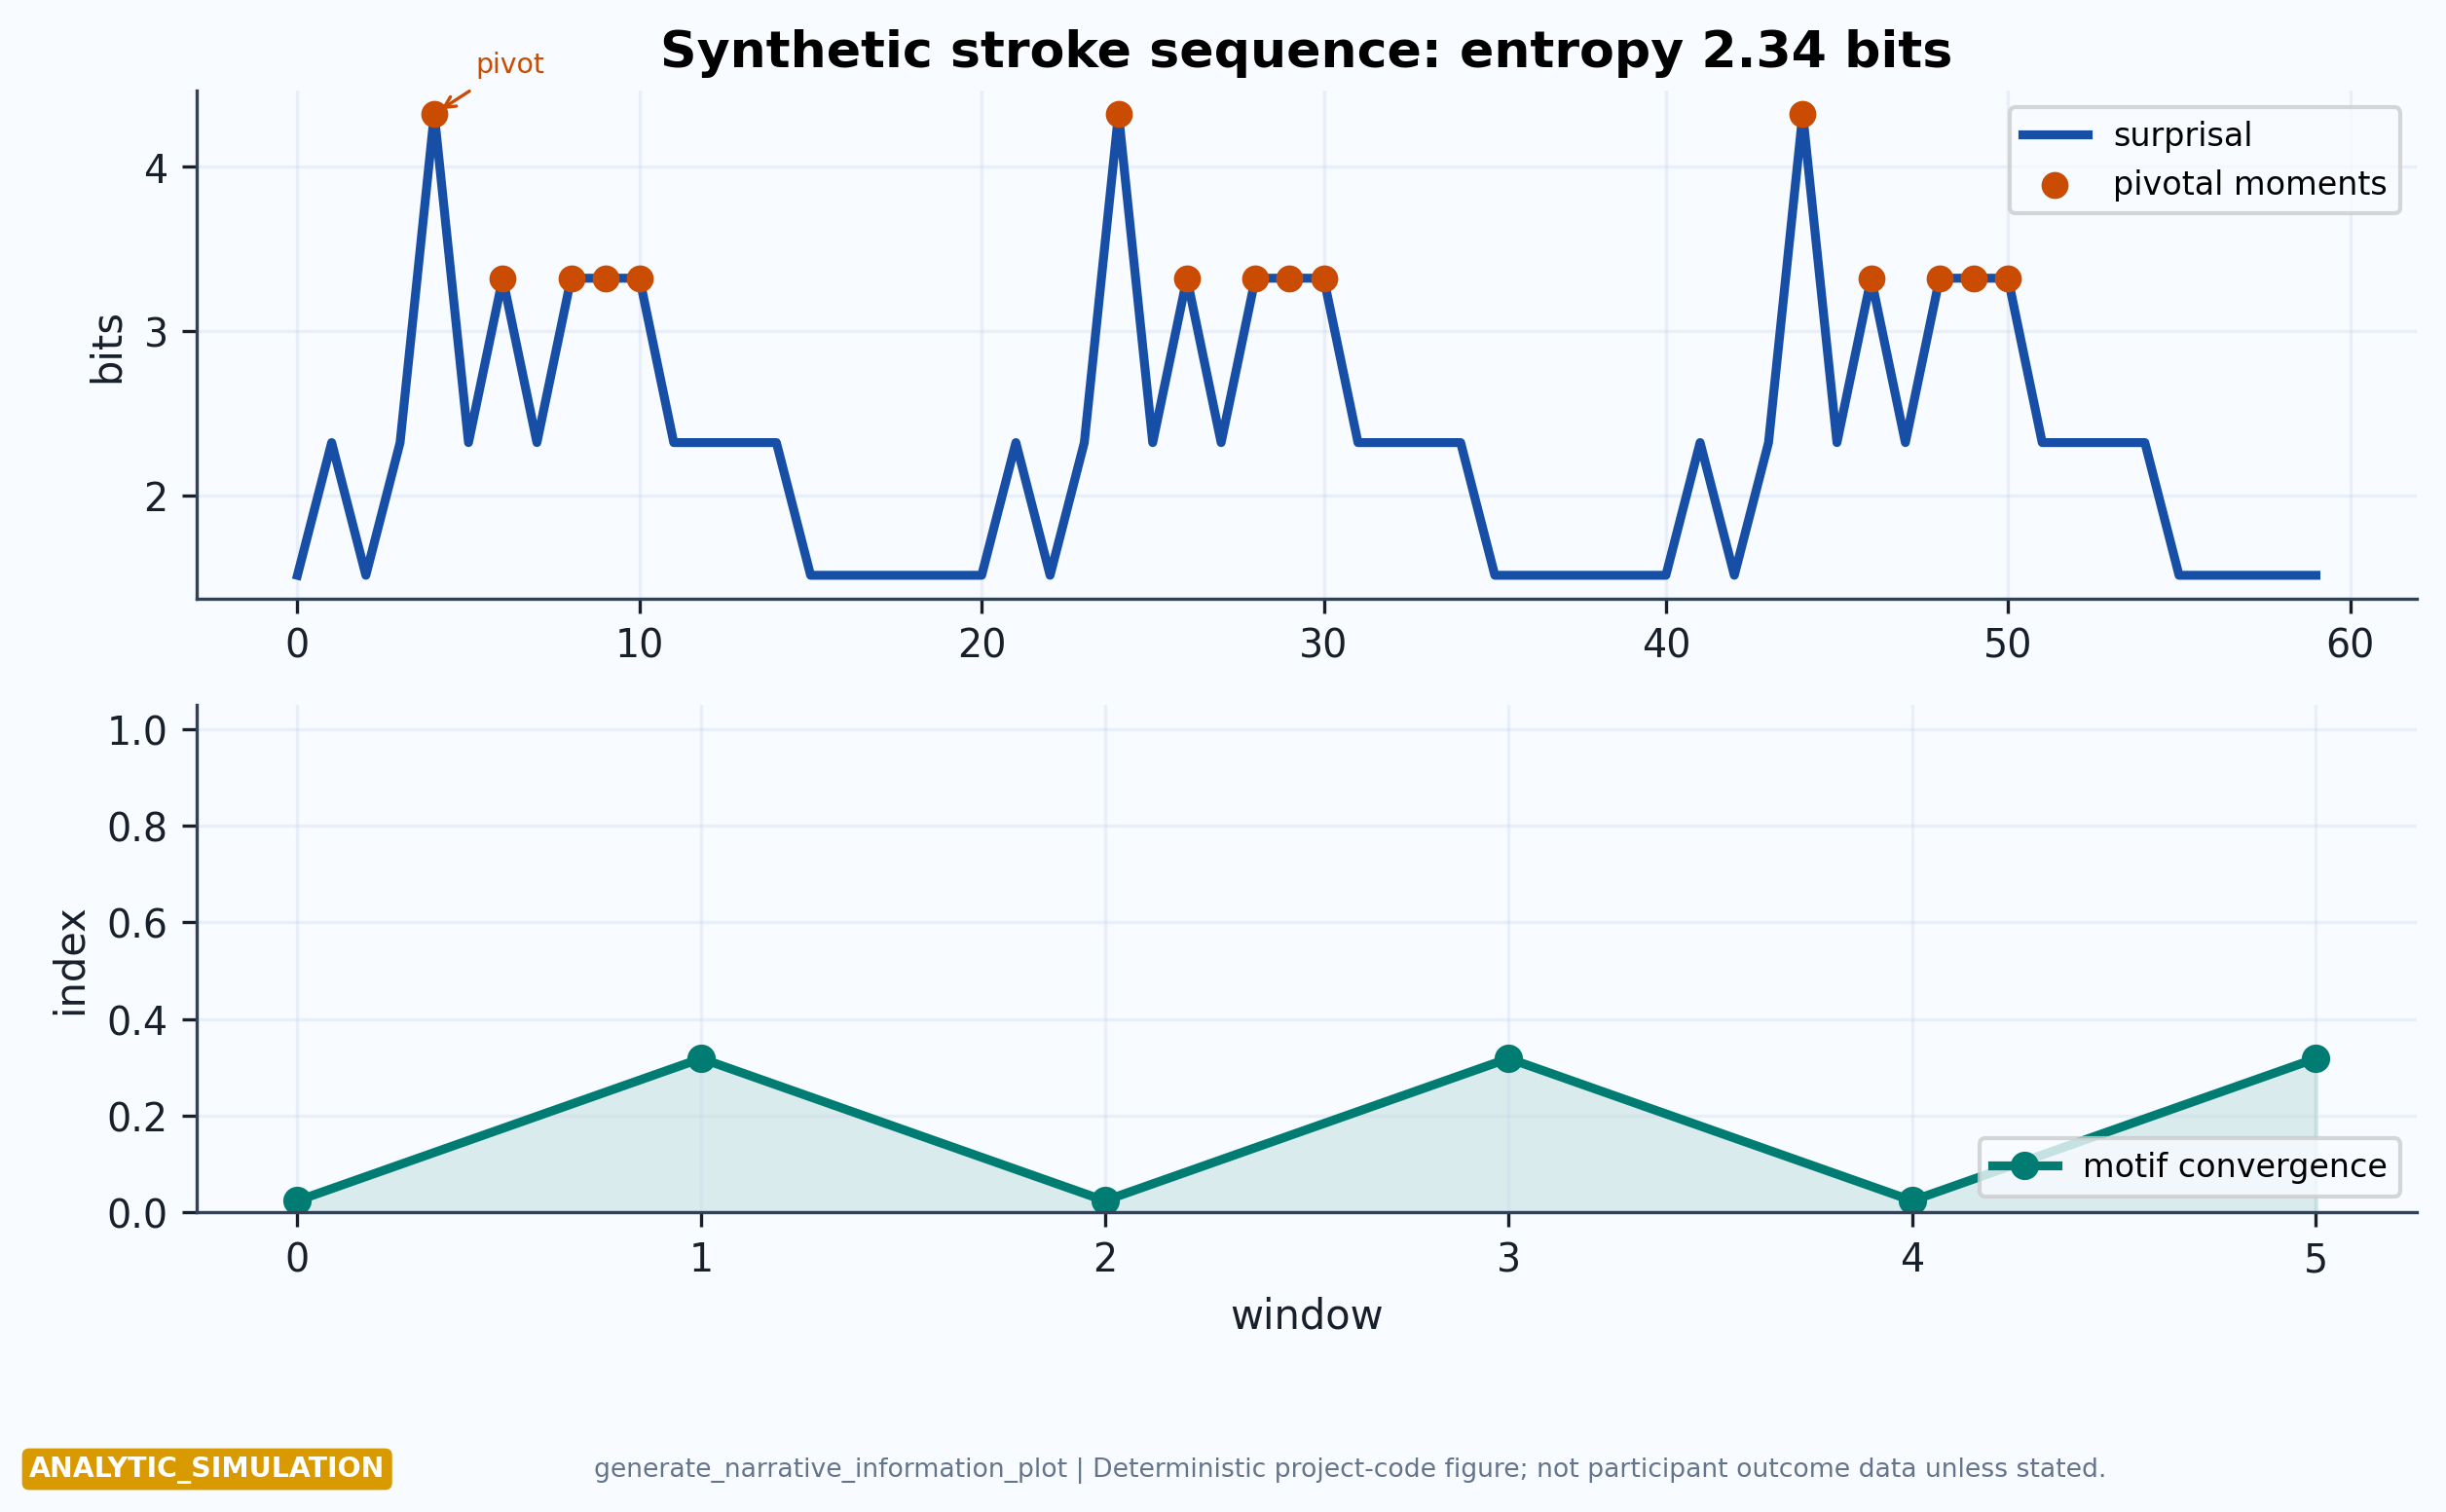
\includegraphics[width=0.9\linewidth,height=0.46\textheight,keepaspectratio,alt={Narrative-information diagnostics for a conceptual stroke sequence. The figure is generated by generate\_narrative\_information\_plot() from src/narrative.py; read the upper panel as surprisal with pivotal-moment markers and the lower panel as convergence toward a repeated motif. It supports the narrative-information appendix by making the entropy primitive inspectable. The sequence is synthetic, and participant claims would require coded stroke alphabets and inter-rater checks.}]{../figures/narrative_information.png}
\caption{Narrative-information diagnostics for a conceptual stroke
sequence. The figure is generated by
\protect\breaktt{generate\_narrative\_information\_plot()} from
\protect\breaktt{src/narrative.py}; read the upper panel as surprisal
with pivotal-moment markers and the lower panel as convergence toward a
repeated motif. It supports the narrative-information appendix by making
the entropy primitive inspectable. The sequence is synthetic, and
participant claims would require coded stroke alphabets and inter-rater
checks.}\label{fig:narrative_information}
\end{figure}

\begin{figure}
\centering
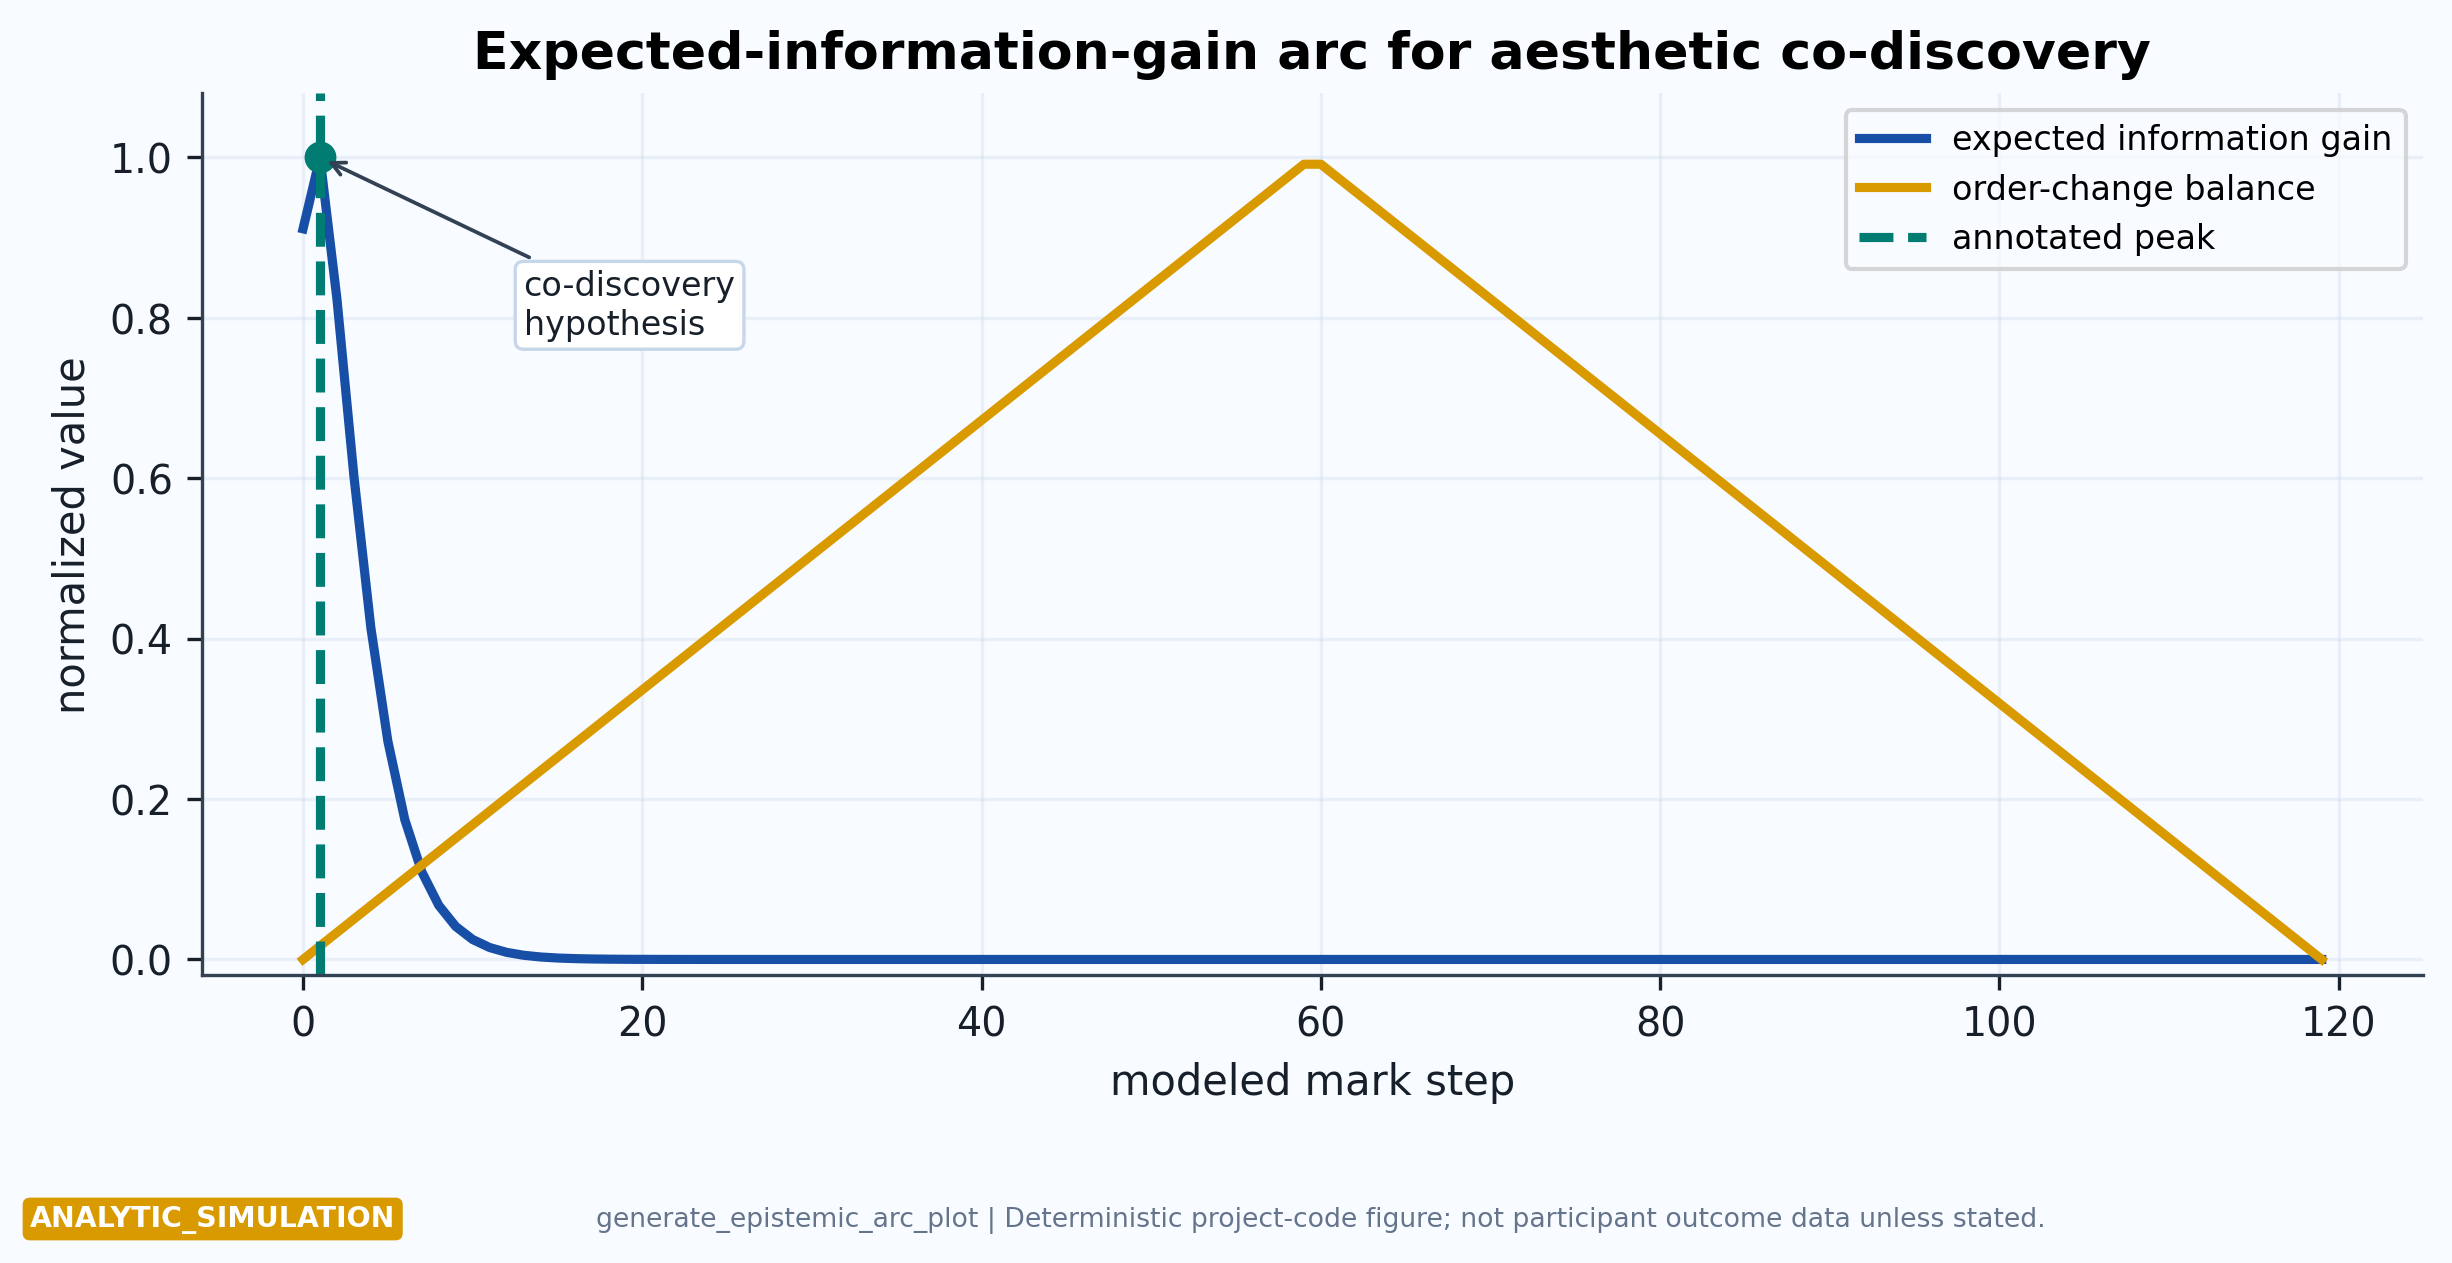
\includegraphics[width=0.9\linewidth,height=0.46\textheight,keepaspectratio,alt={Expected-information-gain and order-change balance in a conceptual DigiPPPiP session. The figure is generated by generate\_epistemic\_arc\_plot() from src/aesthetics.py; read the normalized curves as an illustrative relation between curiosity, order, change, and the marked ``aha'' peak. It supports the appendix's modeling vocabulary. The plot is conceptual, and validation would require event-aligned experience reports or behavioral measures.}]{../figures/epistemic_arc.png}
\caption{Expected-information-gain and order-change balance in a
conceptual DigiPPPiP session. The figure is generated by
\protect\breaktt{generate\_epistemic\_arc\_plot()} from
\protect\breaktt{src/aesthetics.py}; read the normalized curves as an
illustrative relation between curiosity, order, change, and the marked
``aha'' peak. It supports the appendix's modeling vocabulary. The plot
is conceptual, and validation would require event-aligned experience
reports or behavioral measures.}\label{fig:epistemic_arc}
\end{figure}

Together, these equations function as a falsifiable grammar for future
studies. They succeed only if they help specify what should be measured,
what comparison would matter, and what result would count against the
interpretation. A free-energy curve that improves only because of
parameter choices, a synchrony measure that disappears after artifact
controls, or an entropy score unrelated to participant reports would all
narrow the framework rather than embarrass it.
\end{frame}

\end{document}
